%
% Permission is granted to copy, distribute and/or modify this
% document under the terms of the Creative Common by-nc-sa License
% version 3.0 (CC BY-NC-SA 3.0). A copy of the license can be found at
% http://creativecommons.org/licenses/by-nc-sa/3.0/legalcode.
%

\usepackage[french]{babel}
\usepackage{listings}
\usepackage{color}

% Highlight macros
\newcommand{\highlight}[1]{\textcolor{structure.fg}{\bfseries #1}}

%% Title, subtitle, authors, institute, date, ...
\title{Attaques sur SSL/TLS}
\subtitle{Poodle, une application du Padding Oracle Attack}

\author[]{Youri Laforgue\\[-.25em]
        \texttt{\scriptsize <youri.laforgue@etu.u-bordeaux.fr>}\\
        Stewie Suivant\\[-.25em]
        \texttt{\scriptsize <stewie.suivant@etu.u-bordeaux.fr>}}

\institute[Master CSI, France]{Master CSI, Université de Bordeaux, France}

\date{\today}
 
%%%%%%%%%%%%%%%%%%%%%%%%%%[ Document ]%%%%%%%%%%%%%%%%%%%%%%%%%%
\begin{document}

\lstset{language=C}

\begin{frame}
  \vspace{3.5em}
  \titlepage

  \begin{center}
    
\includegraphics[scale=.2]{cc-by-nc-sa.pdf}
  \end{center}
\end{frame}

\begin{frame}
  \frametitle{Plan}
  \tableofcontents[subsectionstyle=hide]
\end{frame}

\begin{frame}
  \frametitle{Présentation}

  \begin{itemize}
  \item Protocole qui sécurise les échanges sur un  réseau
  \item Créer en 1995 par Netscape et actuellement en version TLS 1.2
  \item Il garantie l'authentification, l'intégrité et la confidentialité
  \item Il est largement utilisé et donc victime de nombreuses attaques
  \end{itemize}
\end{frame}

%%%%%%%%%%%%%%%%%%%%%%%%%%%%%%%%%%%%%%%%%%%%%%%%%%%%%%%%%%%%%%%%%%%%%%
\section{Attaques sur SSL/TLS}

\begin{frame}<handout:0>
  \frametitle{Plan}
  \tableofcontents[currentsection]
\end{frame}

\begin{frame}
  \frametitle{Classification }

  \begin{itemize}
  \item Oracle Attack
    \pause
  \item Padding Oracle Attack
    \pause
  \item Timming Attack
    \pause
  \item Compression Attack
    \pause
  \item Other
    \pause
  \end{itemize}
\end{frame}

\begin{frame}
  \frametitle{BEAST}
  \textbf{Pré-requis/Fonctionnement}
  \begin{itemize}
  \item Oracle Attack
  \item Attaque en Man in The Middle
  \item CPA (Choosen plaintext Attack) 
  \item IV connu
  \end{itemize}
\end{frame}

\begin{frame}
  \frametitle{BEAST}
  \begin{figure}[h]
    \centering
  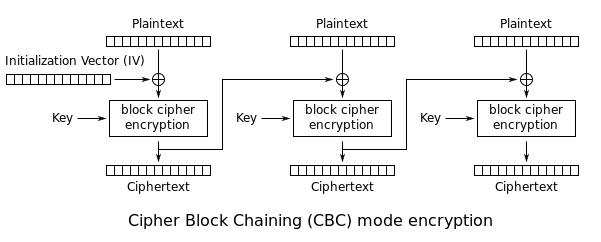
\includegraphics[scale=0.3]{CBC_Encrypt}
  \end{figure}  
\begin{itemize}
  \item  Soit $C = C_1 || C_2 || C_3 || C_4$, un message intercepté par l'attaquant
    \pause
  \item il génère $P' = C_4 + P_3' + C_2 || \dots$
    \pause
  \item  $C' = E(P_3' + C_2 + C_4 + IV) || \dots $
    \pause
  \item $ C' = E(P_3' + C_2) || \dots $
  \end{itemize}
\end{frame}

 
\begin{frame}
  \frametitle{Padding Oracle Attack}
  \textbf{Pré-requis/Fonctionnement}
  \begin{itemize}
  \item Attaque en Man in The Middle
  \item CPA (Choosen plaintext Attack)
  \item Taille du padding connu
  \end{itemize}
\end{frame}

\begin{frame}
  \frametitle{Padding Oracle Attack}
  \begin{figure}[h]
    \centering
  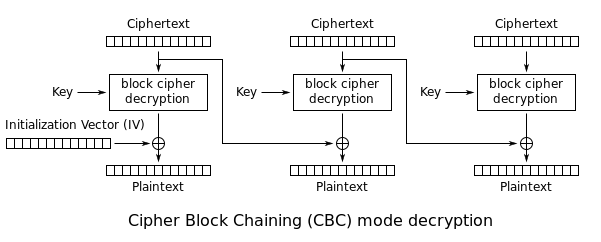
\includegraphics[scale=0.3]{CBC_Decrypt}
  \end{figure}

  \begin{itemize}
  \item  Soit $C = C_1 || C_2 || C_3 || C_4$, un message intercepté par l'attaquant
    \pause
  \item $C_4'=C_2$
    \pause
  \item $C_3'= C_3$ dont le dernier octet est modifié
    \pause
  \item Si le paquet est valide alors $P_2[k] = p + C_1[k] + C_3'[k]$ 
  \end{itemize}

\end{frame}

\begin{frame}

  \frametitle{Lucky 13}
  \textbf{Pré-requis/Fonctionnement}
  \begin{itemize}
  \item Attaque en Man in The Middle
  \item CPA (Choosen plaintext Attack)
  \item Taille du padding connu
  \item Basée sur le temps du vérification du message
  \end{itemize}
\end{frame}

\begin{frame}
  \frametitle{CRIME}
  \textbf{Pré-requis/Fonctionnement}
  \begin{itemize}
  \item Attaque en Man in The Middle
  \item CPA (Choosen plaintext Attack)
  \item Basée sur la compression SSL d'une requête client
  \end{itemize}
\end{frame}

\begin{frame}[fragile]
  \frametitle{CRIME}
  \begin{itemize}
  \item C1 => ATTACKERDATA:x UNKNOWNCOOKIE:y OTHERDATA»
  \item C2 => ATTACKERDATA:y UNKNOWNCOOKIE:y OTHERDATA»
  \end{itemize}
\pause

\begin{block}{Requête forgée par l'attaquant}
\begin{verbatim}
POST / HTTP/1.1
Host: bank.com
(…)
Cookie: sessionid=d8e8fca2dc0f896fd7cb4cb0031ba249
(…)
sessionid=a
\end{verbatim}
\end{block}
\end{frame}

\begin{frame}
  \frametitle{BREACH}
  \textbf{Pré-requis/Fonctionnement}
  \begin{itemize}
  \item Attaque en Man in The Middle
  \item CPA (Choosen plaintext Attack)
  \item Basée sur la taille de compression HTTP d'une réponse serveur
  \end{itemize}
\end{frame}

\begin{frame}[fragile]
  \frametitle{BREACH}

\begin{block}{ Requête forgée par l'ataquant }
\begin{verbatim}
GET /product/?id=1234&user=CSRFtoken=x HTTP/1.1
Host: exemple.fr
(…)
\end{verbatim}
\end{block}

\begin{block}{Réponse HTTP du serveur}
\begin{verbatim}
<form target="https://exemple.fr:443/products/catalogue.a
spx?id=1234&user=CSRFtoken=x HTTP/1.1">
(...)
<td nowrap id="tdErrLgf">
<a href="logoff.aspx?CSRFtoken=4bd634cda846fd7cb4cb0031ba
249ca2">Log Off</a>
</td>
(…)
\end{verbatim}
\end{block}
\end{frame}

\begin{frame}
  \frametitle{Triple Handshake RSA}
  \textbf{Pré-requis/Fonctionnement}
  \begin{itemize}
  \item Client se connecte sur le serveur de l'attaquant
  \item L'attaquant se connecte sur le serveur cible
  \item L'attaque se déroule en trois poignées de main
\end{itemize}
\end{frame}

\begin{frame}
  \frametitle{Triple Handshake RSA}
    \begin{enumerate}
    \item Handshake avec authentification du serveur
      \begin{itemize}
      \item L'attaquant impose RSA
      \item Le client a le certificat de l'attaquant
      \item Les logs du client et du serveur sont différents
      \end{itemize}
      \pause
    \item Handshake abrégé
      \begin{itemize}
      \item L'attaquant forward simplement les paquets
      \item Le client et le serveur partagent les mêmes logs
      \end{itemize}
      \pause
    \item Renégociation complète avec authentification mutuelle
      \begin{itemize}
      \item Le client et le serveur ont les bons certificats
      \item L'attaquant ne connait plus le master secret
      \end{itemize}
    \end{enumerate}

\end{frame}

\begin{frame}
  \frametitle{FREAK}
  \textbf{Pré-requis/Fonctionnement}
  \begin{itemize}
  \item Attaque en Man in The Middle
  \item Forcer le mode de chiffrement avec une clé RSA-Export
  \item Trouver la clé secrète par recherche exhaustive
  \end{itemize}
\end{frame}

\begin{frame}
  \frametitle{Heartbleed}
 Basée sur l'extension Heartbeat
  \begin{figure}[h]
    \centering
  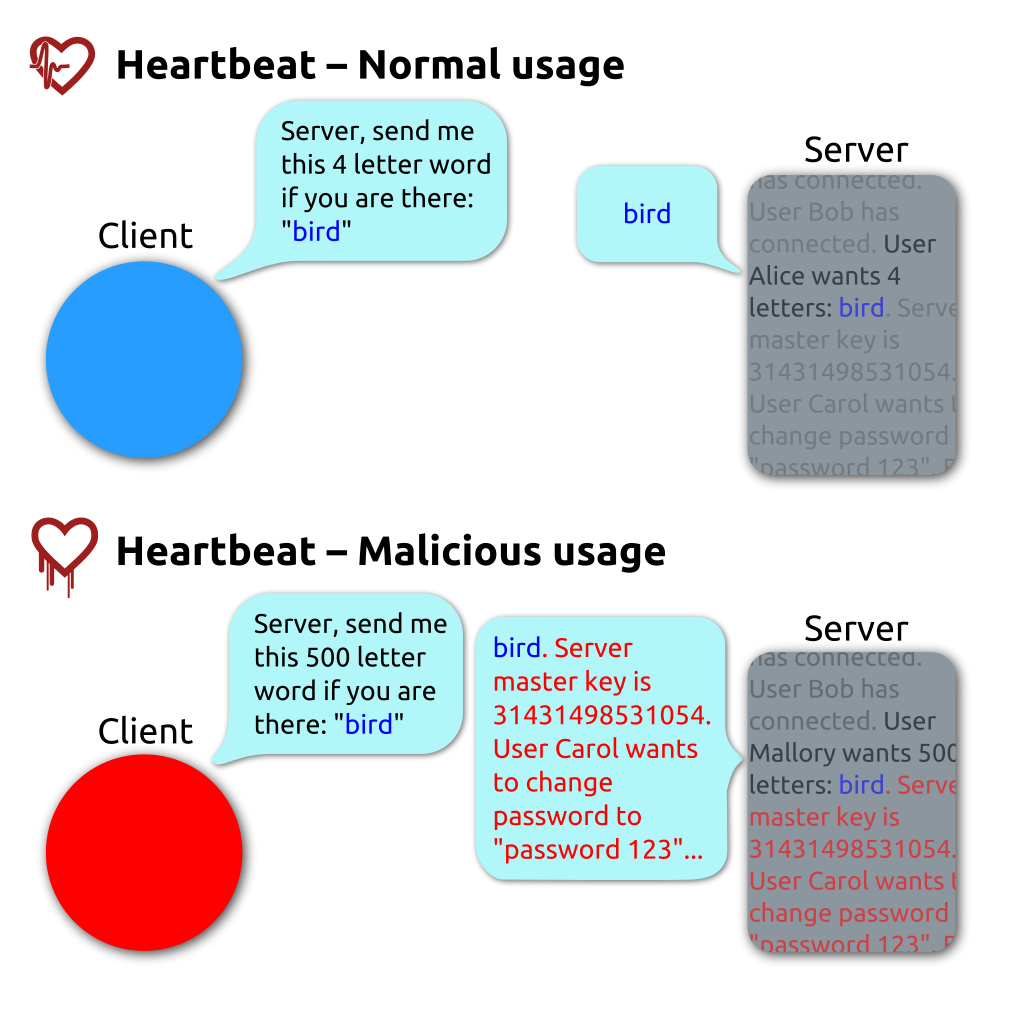
\includegraphics[scale=0.17]{Heartbleed}
  \end{figure}
\end{frame}


%%%%%%%%%%%%%%%%%%%%%%%%%%%%%%%%%%%%%%%%%%%%%%%%%%%%%%%%%%%%%%%%%%%%%%
\section{Poodle}

\begin{frame}<handout:0>
  \frametitle{Plan}
  \tableofcontents[currentsection]
\end{frame}

\begin{frame}
  \frametitle{Présentation}
  Découvert par Bodo Möller, Thai Duong et Krzysztof Kotowicz en Septembre 2014.\\
  \pause
\textbf{Pré-requis/Fonctionnement}
  \begin{itemize}
  \item Basée sur le Padding Oracle Attack
  \item Attaque en Man in The Middle
  \item CPA (Choosen plaintext Attack)
  \item Taille du padding connu
  \end{itemize}

\end{frame}

\begin{frame}
  \frametitle{Paquet SSL}
  \begin{figure}[h]
    \centering
    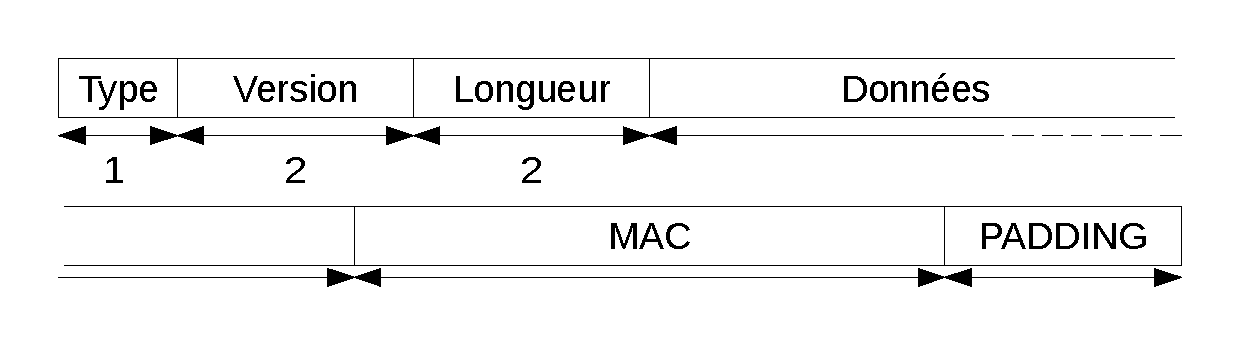
\includegraphics[scale=0.5]{schemaSSL2}
  \end{figure}
  \begin{tabular}{|l|l|l|}
    \hline
  Type  & Version & Mac \\
    \hline
   0x16 : Handshake  &  0x3000 : SSLv3 &  SHA1 : 20 octets\\
   0x14 : Change Cypher Spec &  0x30xy : TLSvx.y & SHA256 : 32 octets\\
   0x15 : Alert & \dots & \dots\\
   0x17 : Application Data  & &\\
    \hline
  \end{tabular}

\end{frame}

\begin{frame}
  \frametitle{Comment ça marche}
  \begin{figure}[h]
    \centering
  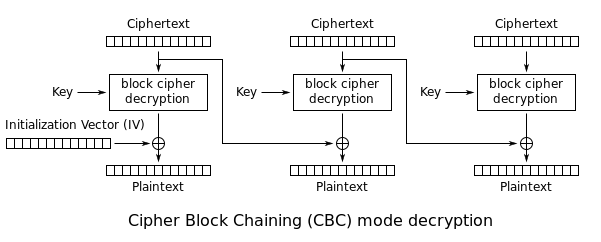
\includegraphics[scale=0.3]{CBC_Decrypt}
  \end{figure}
    \begin{itemize}
  \item  Soit $C = C_1 || C_2 || C_3 || C_4$, un message intercepté par l'attaquant
    \pause
  \item $C_4'=C_2$
    \pause
  \item Si le paquet est valide alors $P_2[k] = p + C_1[k] + C_3[k]$ \\
    Sinon renégociation de la clé
  \end{itemize}
\end{frame}

\begin{frame}
  \frametitle{Implémentations}
  
  \begin{enumerate}
  \item Padding Oracle Attack
    \begin{itemize}
    \item Contexte TCP
    \item Chiffrement DES
    \item environ 150 tentatives par octet
    \end{itemize}
    \pause
  \item Poodle
    \begin{itemize}
    \item Contexte TCP et SSL
    \item Chiffrement DES
    \item environ 350 tentatives par octet
    \end{itemize}
  \end{enumerate}

\end{frame}


\begin{frame}
  \frametitle{Implémentations}
  \begin{block}{Algorithme de POODLE}
    \lstinputlisting[language=C]{test.c}
  \end{block}
\end{frame}


%%%%%%%%%%%%%%%%%%%%%%%%%%%%%%%%%%%%%%%%%%%%%%%%%%%%%%%%%%%%%%%%%%%%%%
\section{Références}

\begin{frame}<handout:0>
  \frametitle{Plan}
  \tableofcontents[currentsection,subsectionstyle=hide]
\end{frame}

\nocite{*}
\bibliographystyle{alpha}

\begin{frame}[allowframebreaks]
  \frametitle{Références}
  \bibliography{bibliography}
\end{frame}

%%%%%%%%%%%%%%%%%%%%%%%%%%%%%%%%%%%%%%%%%%%%%%%%%%%%%%%%%%%%%%%%%%%%%%
\begin{frame}
  \vfill
  \centering
  \highlight{\Huge Questions~?}
  \vfill
\end{frame}
